\subsubsection{Evolution}

evolve without great effort.

We argue that a goal model can be seen as a protocol definition. When we create OR-Refinements we are giving alternatives of execution, creating variability points.

By creating interfaces in variability points
Open deployment platform.

  and we create opportunity for thirty-parties provide new alternativies

having different context condition will allow the goal to be achievable in a broader range of contexts: for example, in screen controls will allow the game to be playable at touch screen devices.

In tradition deployment schema, a complete new version of the software should be released.

\begin{figure}[!htb]
  \centering
  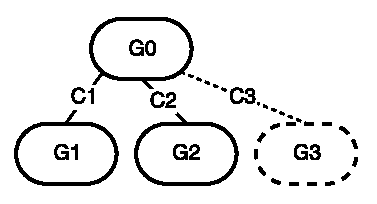
\includegraphics[width=\linewidth]{evolution_or}
  \caption{Evolution OR}
\label{fig:evolution_or}
\end{figure}

Component development and release
